\section{Correção da distorção}

Os parâmetros de cada câmera foram reutilizados em \texttt{undistort.py} para
corrigir a distorção geométrica com \texttt{cv2.undistort()}. A função
\texttt{cv2.}\allowbreak\texttt{getOptimalNewCameraMatrix()} determina uma nova matriz
intrínseca para a mesma resolução, com duas escolhas de
$\alpha$~\cite{opencv-tutorial}. Para $\alpha=0$, prioriza-se uma região válida,
evitando bordas pretas e reduzindo o campo de visão. Para $\alpha=1$, preserva-se
mais do campo original, com possíveis regiões sem pixels correspondentes,
representadas em preto. O programa não recorta a região de interesse retornada
nem redimensiona os arquivos corrigidos.

Foram utilizadas fotografias de teste sem tabuleiro, separadas das imagens de
calibração. As Figuras~\ref{fig:undistort1} e~\ref{fig:undistort05} reproduzem
comparações já geradas para \texttt{fogao1.jpg}. As bordas da porta e os rejuntes
dos azulejos, próximos aos limites das fotografias, permitem inspecionar
visualmente as alterações. Cada câmera observa a cena com enquadramento próprio;
a comparação relevante ocorre entre as versões da mesma fotografia.

\begin{figure}[H]
  \centering
  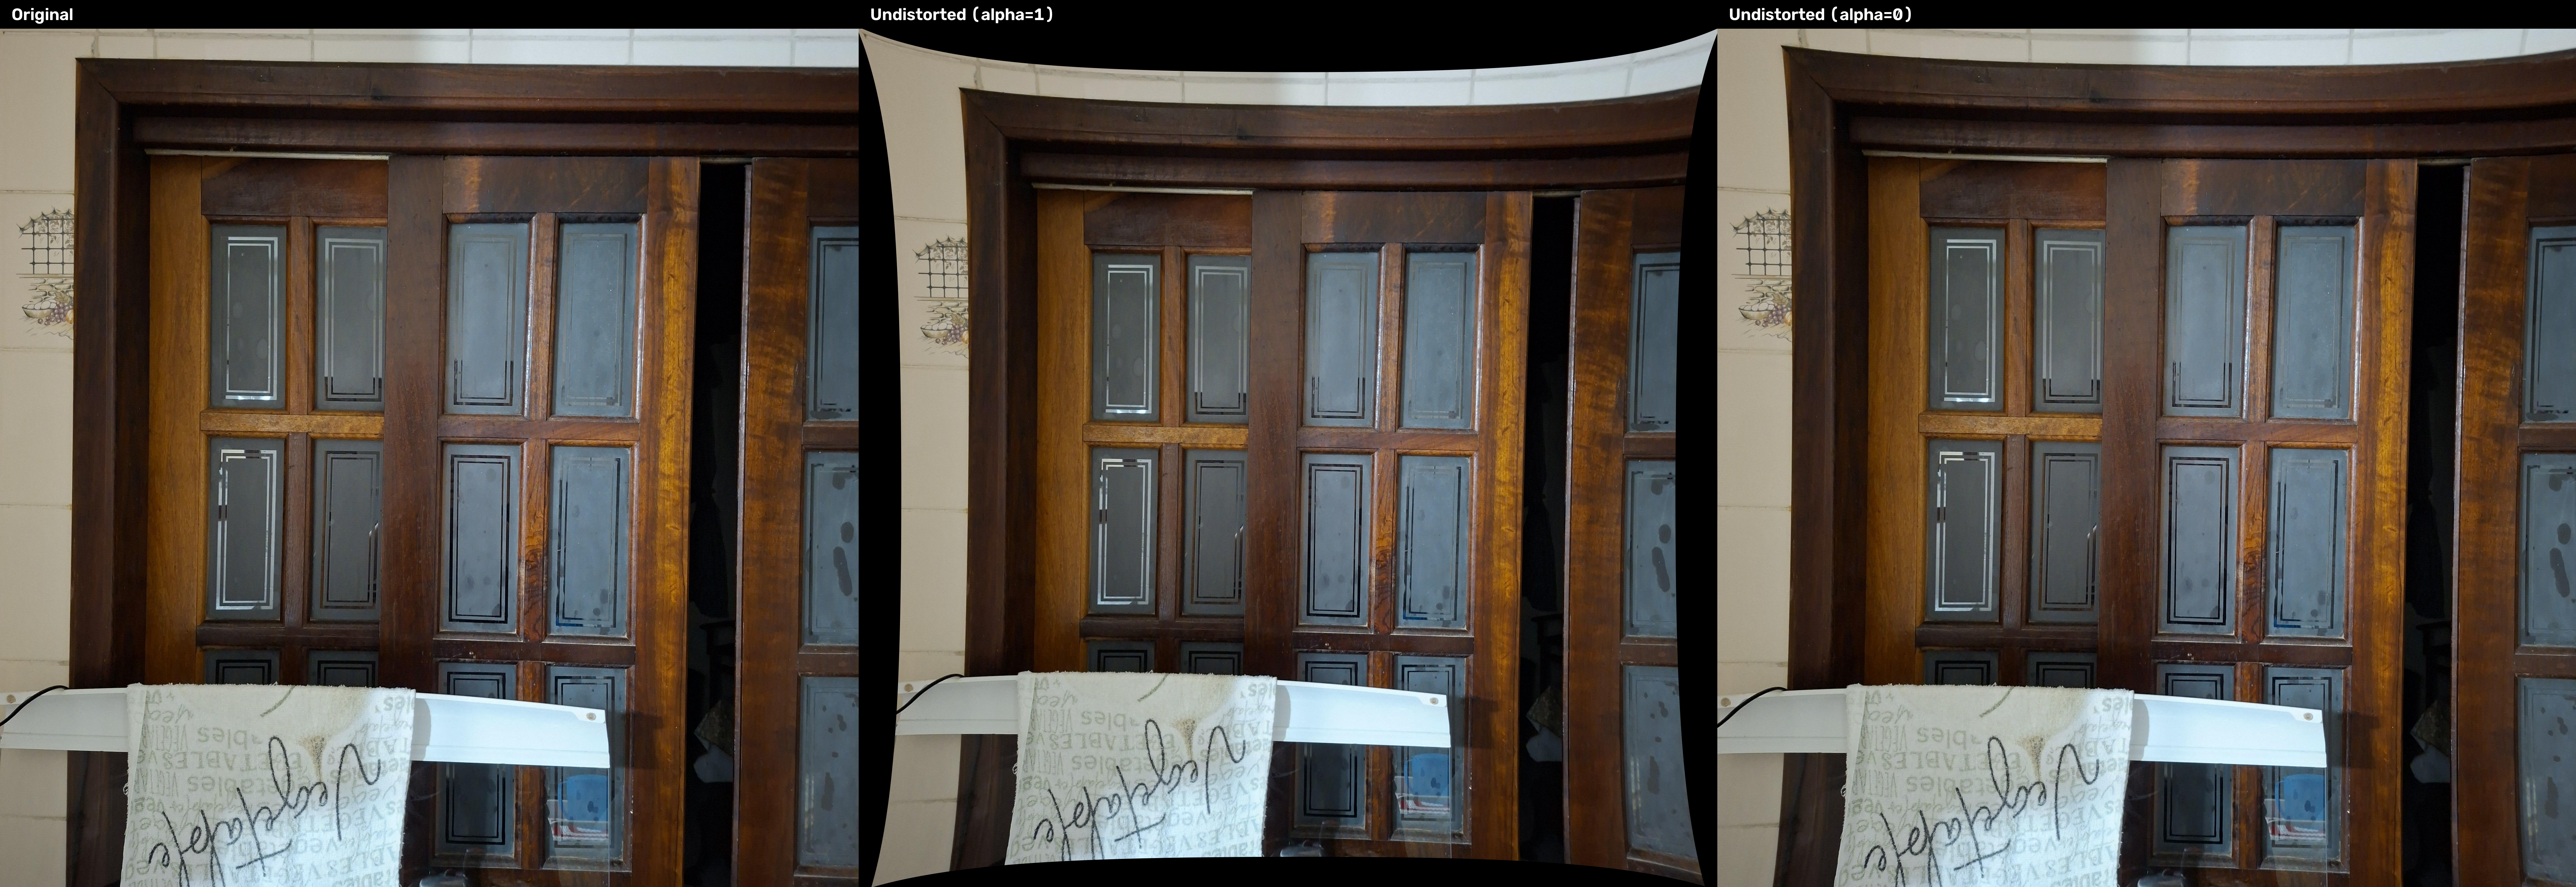
\includegraphics[width=\linewidth]{undistortion-cam1.jpg}
  \caption{Câmera principal (1x), fotografia de teste \texttt{fogao1.jpg}.
  Da esquerda para a direita: original, corrigida com $\alpha=1$ e corrigida
  com $\alpha=0$. A faixa preta curva na versão central corresponde a regiões
  sem amostras da imagem original.}
  \label{fig:undistort1}
\end{figure}

\begin{figure}[H]
  \centering
  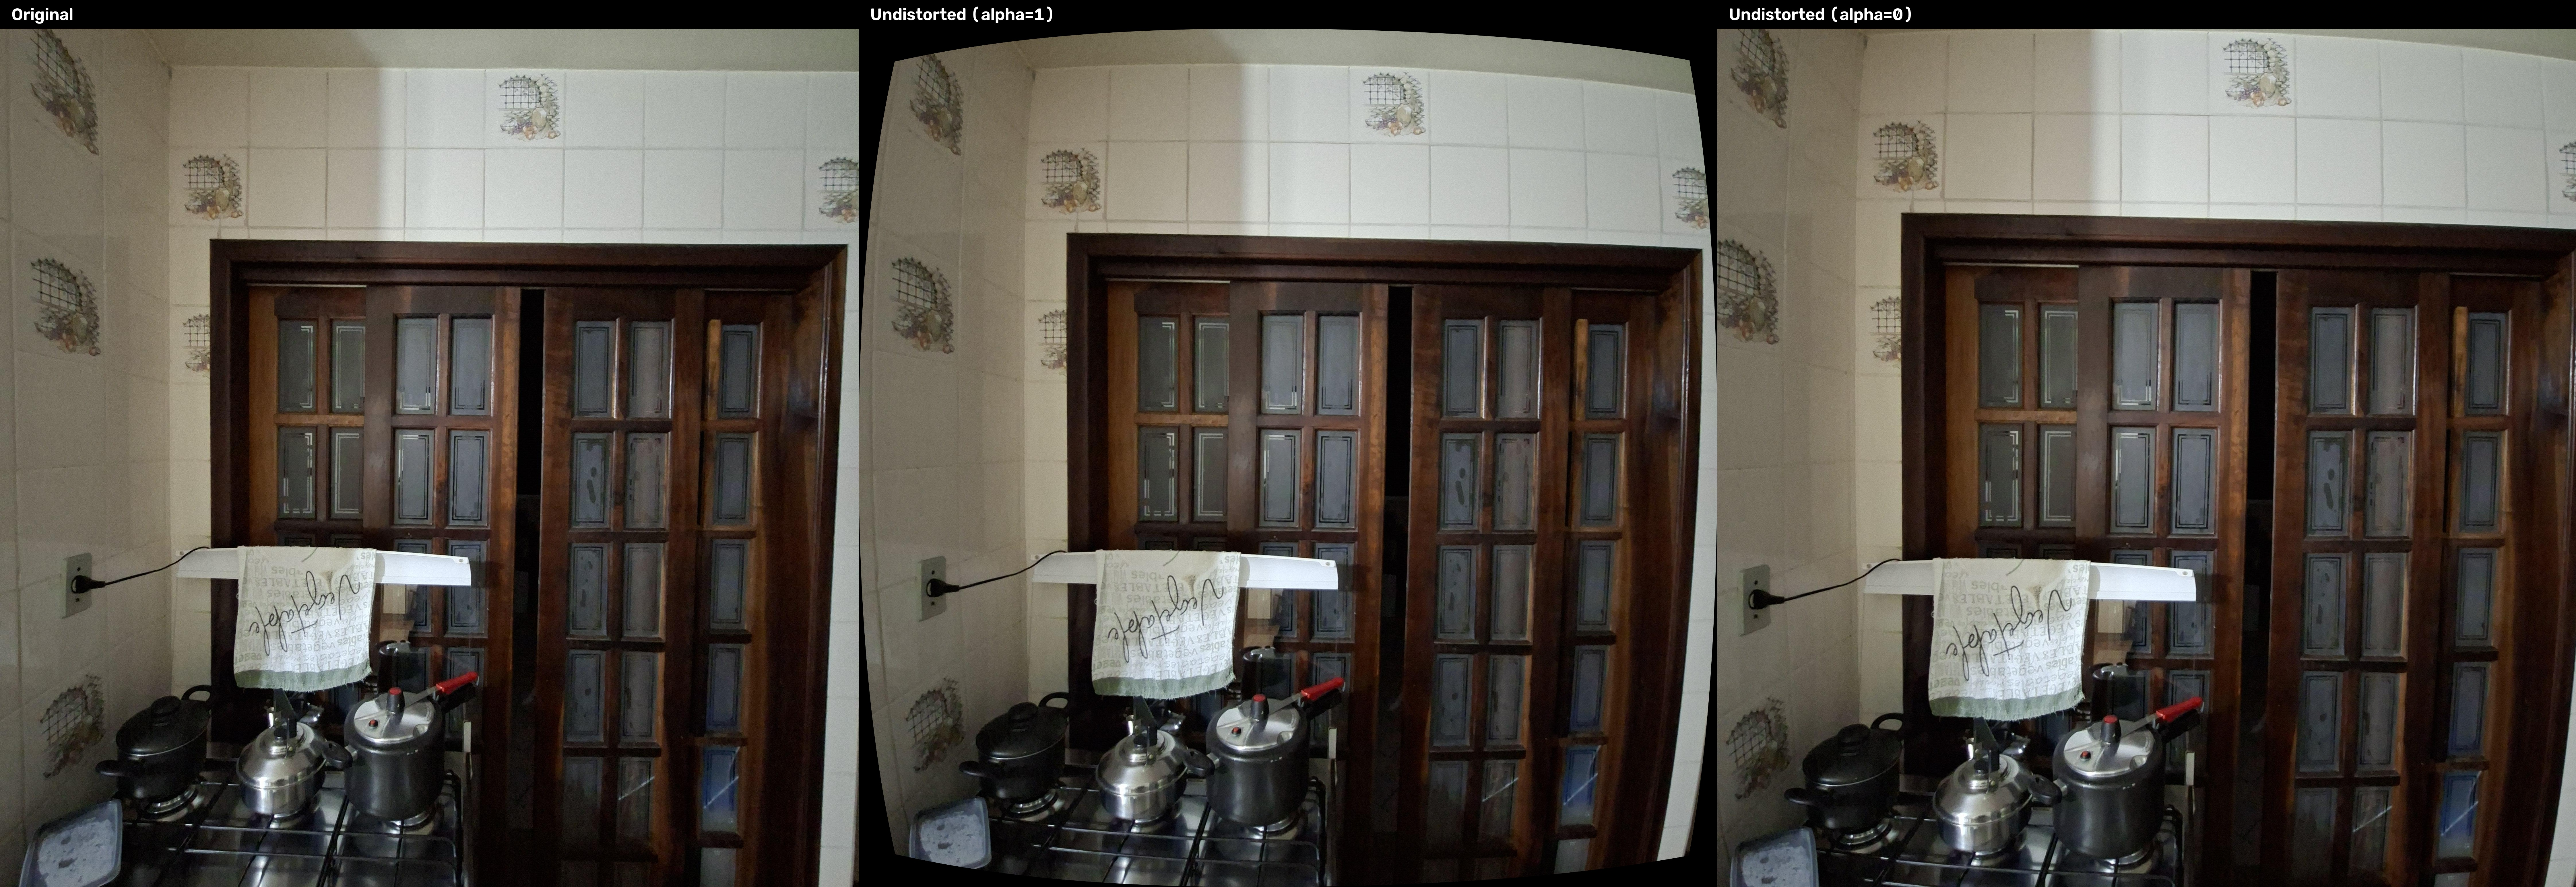
\includegraphics[width=\linewidth]{undistortion-cam05.jpg}
  \caption{Câmera ultrawide (0,5x), fotografia de teste \texttt{fogao1.jpg}.
  A ordem é original, $\alpha=1$ e $\alpha=0$. Observam-se o remapeamento da
  cena, as bordas sem correspondência e a mudança de enquadramento.}
  \label{fig:undistort05}
\end{figure}

As diferenças locais podem ser discretas, embora a alteração de enquadramento
seja visível. Não foi medida a retidão das linhas ou outra métrica geométrica
nas imagens de teste; portanto, essas figuras não demonstram uma melhoria
quantitativa da geometria. A correção também não elimina efeitos de
perspectiva, como a convergência de linhas associada à orientação da câmera em
relação à cena. Bordas pretas, por sua vez, decorrem do domínio do remapeamento
e não representam regiões adicionais capturadas pela câmera.
